\section{Experiments of planning grasps for familiar objects}
\label{cha3:sec3}

This section presents a few results of our method (Figure~\ref{contour},~\ref{icub_cuboid}\footnote{The small penetrations and gaps between the fingers and the object are caused by two factors, (1) that the width of the fingers are not taken into account in the optimization and (2) the variance of the results. A supplemental implementation will be applied on the real scenario to handle the variances.},~\ref{barrett}). As mentioned above, grasps of the iCub hand are described in 14 dimensions: hand position (3D), hand orientation (3D in Euler angles) and finger joint angles (8D). Grasps of the Barrett hand are described in 8 dimensions: hand position (3D), hand orientation (4D in axis-angle representations) and finger separation angle (1D). Six different objects are presented here: cylinder, cuboid, ashtray, shoe, joystick and aeroplane model. For each object, three different initial postures and their final grasps are shown. Figure~\ref{contour} shows the results of the iCub grasping a cylinder, and the corresponding projections from the initial query points to the model. The results of the cylinder and cuboid show that a variety of grasps can be obtained for simple shapes to satisfy different task requirements. The ashtray, aeroplane model and joystick shapes are chosen from the GraspIt! object library, showing the method indeed works with complex shapes. In some figures the wrist may seem to rotate over 360 degrees to reach the final grasps from the initial pose. This is because the path planning of the arm is not taken into account in our approach. In terms of the hand orientation solely, a much smaller rotation is needed to go from the initial pose to the final grasp.

\begin{figure}

  \centering
  \subfloat[\scriptsize{Initial pose 1}]  {\label{fig:reachableSamplesPos}\includegraphics[width=4cm]{./fig_cha3/1_ini.png}}
  \subfloat[\scriptsize{Initial pose 2}] {\label{fig:reachableModelPos}  \includegraphics[width=4cm]{./fig_cha3/2_iniss.png}}
  \subfloat[\scriptsize{Initial pose 3}]  {\label{fig:reachableSamplesPos}\includegraphics[width=4cm]{./fig_cha3/aa.png}}

  \vspace{0.02in}
  \subfloat[\scriptsize{Final grasp 1}] {\label{fig:reachableSamplesPos}\includegraphics[width=4cm]{./fig_cha3/1_finalss.png}}
  \subfloat[\scriptsize{Final grasp 2}] {\label{fig:reachableModelPos}  \includegraphics[width=4cm]{./fig_cha3/2_finalss.png}}
  \subfloat[\scriptsize{Final grasp 3}]  {\label{fig:reachableSamplesPos}\includegraphics[width=4cm]{./fig_cha3/3_final_2ss.png}}

  \vspace{0.2in}
  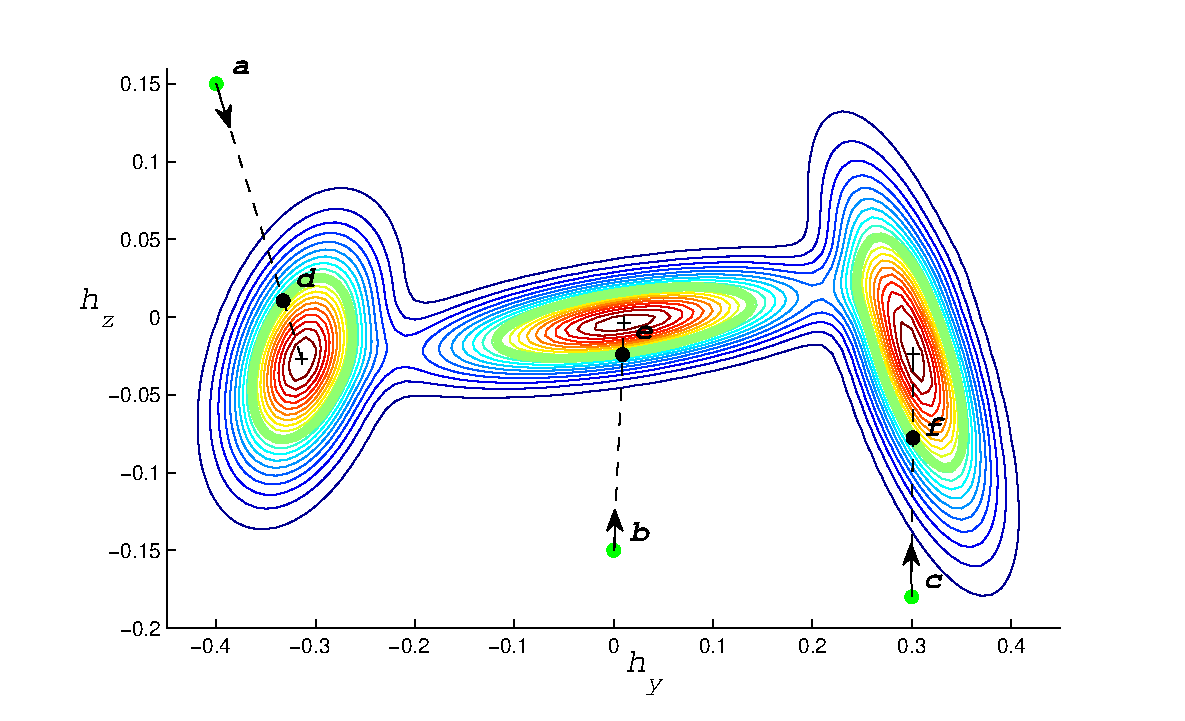
\includegraphics[width=14cm]{./fig_cha3/contour2-3_4.eps}
  \caption{\scriptsize{
  Two-dimensional illustration of the learned model. $h_y$ and $h_z$ correspond to the hand position along the y and z axis of the object reference frame. a, b and c are the initial query points, while d, e and f are their corresponding computed grasps.
  Green dots correspond to initial query inputs  {\bf {\em q}}, black dots correspond to found feasible query inputs {\bf {\em q}}$^*$, contours correspond to parts of the space with constant likelihood, and the thick green contours correspond to threshold values $\eta$ = exp(-$\frac{1}{2}\sigma^2$) of each Gaussian, where $\sigma = 1$ standard deviations.
  The initial finger joint angles in a,b,c are all set to zero. After each feasible query point is found, GMR is used to predict the finger configuration to get the final grasp d,e,f. }
}
    \label{contour}
\end{figure}


\begin{figure}
  \centering
    \subfloat[\scriptsize{Initial pose 1}]  {\label{fig:reachableSamplesPos}\includegraphics[width=5cm]{./fig_cha3/cuboid_1_i.pdf}}
    \subfloat[\scriptsize{Initial pose 2}] {\label{fig:reachableModelPos}  \includegraphics[width=5cm]{./fig_cha3/cuboid_2_i.pdf}}
    \subfloat[\scriptsize{Initial pose 3}] {\label{fig:reachableModelPos}  \includegraphics[width=5cm]{./fig_cha3/cuboid_3_i.pdf}}

    %\vspace{0.05in}

    \subfloat[\scriptsize{Final grasp 1}] {\label{fig:reachableModelPos}  \includegraphics[width=5cm]{./fig_cha3/cuboid_1_f.pdf}}
    \subfloat[\scriptsize{Final grasp 2}]  {\label{fig:reachableSamplesPos}\includegraphics[width=5cm]{./fig_cha3/cuboid_2_f.pdf}}
    \subfloat[\scriptsize{Final grasp 3}]  {\label{fig:reachableSamplesPos}\includegraphics[width=5cm]{./fig_cha3/cuboid_3_f.pdf}}

  \caption{\scriptsize{Examples of the iCub hand grasping a cuboid. The first row (a,b,c) shows the initial postures and the second row (d,e,f) shows the corresponding final grasps.}
}
    \label{icub_cuboid}
\end{figure}

To test the computation time we generated 3000 random initial query points for each grasping task. The initial query points are placed at different distances away from the object surface, varying between 3$cm$ to 50$cm$, and the hand orientation is random. The initial finger configuration is not taken into account in finding the feasible region and hence it is set to the robot hand starting values. The computation time and experimental details are shown in Table~\ref{result}.

Table~\ref{result} also shows the success rate of generated grasps with the iCub and the Barrett hand. A grasp is considered to be successful if it satisfies the force-closure criterion, is feasible for the hand kinematics and is not in collision with the object (see Section~\ref{cha3:sec2:demonstration}). When executing the obtained grasp, the fingers will continue to clutch until contact is made; if they contact the object surface before reaching the expected finger configuration, they will halt to avoid penetration.
All the results shown in Figure.~\ref{contour},~\ref{icub_cuboid},~\ref{barrett} are good grasps.

As can be seen from Table~\ref{result}, the success rate depends on the dimensions of the grasp space and the surface geometry of the target objects. Grasps in lower degrees of freedom (the Barrett hand) have higher success rates than those in higher degrees of freedom (the iCub hand). This suggests that the higher dimension grasp space is more complex than the lower dimension grasp space and needs more data to represent the full complexity. On the other hand, objects with smooth surfaces have a success rate around 90\%. Objects with a couple of prominences have success rates over 85\% as the configuration space of grasping is discontinuous. In the Barrett hand and aeroplane model task, the failed grasps are concentrated on two places: the thin edges of the wings and the propeller. Grasping these places requires high accuracy and more training data on these parts would be needed.
%On the other hand, objects with smooth surface have a high rate of success. Objects with a couple of prominence have success rate about 85\% as the configuration space of grasping is discontinue. In the Barrett hand and airplane model task, the failure grasps are concentrated on two places: the thin edges of the wings and the propeller. Grasping these two places require high accuracy and this is not the main concern of this paper.

To compare with the training data, we compute the grasp quality of the results with the same metrics we used in data generation. The mean of the grasp quality of the training set and the result set are similar, though the result set has a slightly higher value in most of cases. We are able to find some grasps of higher quality than all grasps in the training set (Figure~\ref{near}). This shows that GMM is able to model and generalize the high dimensional grasp space, especially for objects with smooth surfaces.

% For the iCub hand, 612 different feasible grasps of a cylindrical object are obtained by the optimization~\citep{sahar2012}. The learned GMM model has 40 Gaussian components, determined by BIC, and each Gaussian has 14 dimensions: hand position (3D), hand orientation (3D), finger joint angles (8D).



\begin{figure}
  \centering
   \subfloat[\scriptsize{Best grasp found. Quality is 0.16. }]  {\includegraphics[width=3cm]{./fig_cha3/ash_near1.pdf}}
   \subfloat[\scriptsize{Best grasp found. Quality is 0.19.}] {\includegraphics[width=3cm]{./fig_cha3/joy_near1.pdf}}
   \subfloat[\scriptsize{Neighbor grasp of (a). Quality is 0.027.}] {\includegraphics[width=3cm]{./fig_cha3/ash_near2.pdf}}
   \subfloat[\scriptsize{Neighbor grasp of (b). Quality is 0.03.}] {\includegraphics[width=3cm]{./fig_cha3/joy_near2.pdf}}

 \caption{\scriptsize{(a) The best grasp found for the Barrett hand and the ashtray. (b) The best grasp found for the Barrett hand and the joystick. (c) The nearest grasp of (a) in the training set. Note the gap between the finger and the object. (d) The nearest grasp of (b) in the training set. }
}
    \label{near}
\end{figure}


\begin{table*}
\centering
\renewcommand{\arraystretch}{1.5}
    \caption{Average computation time for generating new grasps for the iCub hand and the Barrett hand.}
    \begin{tabular}{|>{\centering\arraybackslash}p{3cm}|>{\centering\arraybackslash}p{1.2cm}|>{\centering\arraybackslash}p{1.7cm}|>{\centering\arraybackslash}p{1.2cm}|>{\centering\arraybackslash}p{1.5cm}|>{\centering\arraybackslash}p{1.5cm}|>{\centering\arraybackslash}p{1.7cm}|>{\centering\arraybackslash}p{1.7cm}|>{\centering\arraybackslash}p{0.9cm}|}%{ | c | c | c | c | c | c | c | c |p{1cm} |}
    \hline
    Robot/Object & Number of training data & Average Grasp Quality(train)& Number of Gaussians& Force-Closure Grasp Found & Average Grasp Quality(result)& Mean of Computation Time($msec$) & Variance ($msec$)   \\ \hline
    iCub/Cylinder       & 621   & 0.0965& 40    & 90\%  & 0.1008    & 9.1   & 0.0001 \\ \hline
    iCub/Cuboid         & 532   & 0.1317& 40    & 89\%  & 0.1224    & 9.4   & 0.0007 \\ \hline
    Barrett/Ashtray     & 1560  & 0.0975& 15    & 100\% & 0.1644    & 4.3   & 0.0001 \\ \hline
    Barrett/Shoe        & 629   & 0.0019& 25    & 99\%  & 0.0034    & 6.9   & 0.0001 \\ \hline
    Barrett/Joystick    & 1500  & 0.0061& 20    & 98\%  & 0.0064    & 5.9   & 0.0002 \\ \hline
    Barrett/Plane       & 1374  & 0.0002& 55    & 85\%  & 0.0003    & 15.1  & 0.0003 \\ \hline

    \end{tabular}

    \label{result}

\end{table*}


\begin{figure*}
  \centering

    \subfloat[\scriptsize{Initial pose 1}]  {\includegraphics[width=5cm]{./fig_cha3/bar_i_1.pdf}}
    \subfloat[\scriptsize{Initial pose 2}] { \includegraphics[width=5cm]{./fig_cha3/bar_i_2.pdf}}
    \subfloat[\scriptsize{Initial pose 3}] { \includegraphics[width=5cm]{./fig_cha3/bar_i_3.pdf}}
    \vspace{0.3in}
    \subfloat[\scriptsize{Final grasp 1}] {\includegraphics[width=5cm]{./fig_cha3/bar_f_1.pdf}}
    \subfloat[\scriptsize{Final grasp 2}]  {\includegraphics[width=5cm]{./fig_cha3/bar_f_2.pdf}}
    \subfloat[\scriptsize{Final grasp 3}]  {\includegraphics[width=5cm]{./fig_cha3/bar_f_3.pdf}}
    \vspace{0.3in}
    \subfloat[\scriptsize{Initial pose 4}]  {\includegraphics[width=5cm]{./fig_cha3/shoe_1i.pdf}}
    \subfloat[\scriptsize{Initial pose 5}] {\includegraphics[width=5cm]{./fig_cha3/shoe_2i.pdf}}
    \subfloat[\scriptsize{Initial pose 6}]  {\includegraphics[width=5cm]{./fig_cha3/shoe_3i.pdf}}
    \vspace{0.3in}
    \subfloat[\scriptsize{Final grasp 4}] {\includegraphics[width=5cm]{./fig_cha3/shoe_1f.pdf}}
    \subfloat[\scriptsize{Final grasp 5}] {\includegraphics[width=5cm]{./fig_cha3/shoe_2f.pdf}}
    \subfloat[\scriptsize{Final grasp 6}]  {\includegraphics[width=5cm]{./fig_cha3/shoe_3f.pdf}}

  \caption{\scriptsize{Examples of Barrett hand grasping different objects (ashtray, shoe, joystick, aeroplane model).
\textcolor{red}{I see no aeroplane model grasping in these images. I think this may be a layout problem as the figure below does include aeroplane images.} 
 The first and third rows (a,b,c,d,e,f and m,n,o,p,q,r) show the initial postures and the second and forth rows (g,h,i,j,k,l and s,t,u,v,w,x) show the corresponding final grasps.}
}
    \label{barrett}
\end{figure*}

\begin{figure*}
  \centering
    \subfloat[\scriptsize{Initial pose 7}]  {\includegraphics[width=5cm]{./fig_cha3/joy_2_i.pdf}}
    \subfloat[\scriptsize{Initial pose 8}] {\includegraphics[width=5cm]{./fig_cha3/joy_3_i.pdf}}
    \subfloat[\scriptsize{Initial pose 9}] {\includegraphics[width=5cm]{./fig_cha3/joy_5_i.pdf}}
    \vspace{0.3in}
    \subfloat[\scriptsize{Final grasp 7}] {\includegraphics[width=5cm]{./fig_cha3/joy_2_f.pdf}}
    \subfloat[\scriptsize{Final grasp 8}]  {\includegraphics[width=5cm]{./fig_cha3/joy_3_f.pdf}}
    \subfloat[\scriptsize{Final grasp 9}]  {\includegraphics[width=5cm]{./fig_cha3/joy_5_f.pdf}}
    \vspace{0.3in}
    \subfloat[\scriptsize{Initial pose 10}]  {\includegraphics[width=5cm]{./fig_cha3/plane_2i.pdf}}
    \subfloat[\scriptsize{Initial pose 11}] {\includegraphics[width=5cm]{./fig_cha3/plane_3i.pdf}}
    \subfloat[\scriptsize{Initial pose 12}] {\includegraphics[width=5cm]{./fig_cha3/plane_1i.pdf}}
    \vspace{0.3in}
    \subfloat[\scriptsize{Final grasp 10}] {\includegraphics[width=5cm]{./fig_cha3/plane_2f.pdf}}
    \subfloat[\scriptsize{Final grasp 11}]  {\includegraphics[width=5cm]{./fig_cha3/plane_3f.pdf}}
    \subfloat[\scriptsize{Final grasp 12}]  {\includegraphics[width=5cm]{./fig_cha3/plane_1f.pdf}}

  \caption{\scriptsize{Examples of Barrett hand grasping different objects (ashtray, shoe, joystick, airplane model). The first and third rows (a,b,c,d,e,f and m,n,o,p,q,r) show the initial postures and the second and forth rows (g,h,i,j,k,l and s,t,u,v,w,x) show the corresponding final grasps.}
}
    \label{barrett2}
\end{figure*}



This approach provides a good estimation of a stable and feasible grasp for the given object and robot hand. In contrast to the common approach of learning from human demonstrations, these grasps are generated solely according to the mechanics of the robot hand. Some resulting grasps are markedly different from  human grasps, especially for the Barrett hand which is very different from the human hand. Our method may therefore out-perform human demonstrations in some contexts by better exploiting differences between human and robot ``physiology''.

To model the actual contact points between the robot hand and the object is difficult in real time because of the high dimensionality of the solution space and the non-linearity of the kinematic constraints. In our method, instead of computing the actual contact point position, we compute the most likely solution using a GMM. Though a certain amount of accuracy is traded off to achieve the real time goal, the overall performance is satisfying. In the experiments listed above, over 90 percent of the testing points find good grasps within a few milliseconds. This method is most efficient for objects with a smooth surface. For complex objects this method can achieve a high success rate of over 85\%. When grasping the parts requiring high precision, additional feedback from visual or tactile sensors is needed for further refinement of the grasp.

This approach requires the object model to be pre-trained. This is to say, we can only plan grasps for familiar objects with this method. It is useful for a robot working in a controlled environment with a limited number of objects, such as in operating theatres. For domestic service robots, however, this is not enough. New objects will continuously come to the house and hence the robot has to be able to grasp novel object shapes. An extension of this method to work on novel objects is discussed in the next two sections.

%The way we project the initial query point to the closest Gaussian component is more conservative.


